\documentclass{sigchi}

% Use this command to override the default ACM copyright statement (e.g. for preprints). 
% Consult the conference website for the camera-ready copyright statement.


%% EXAMPLE BEGIN -- HOW TO OVERRIDE THE DEFAULT COPYRIGHT STRIP -- (July 22, 2013 - Paul Baumann)
% \toappear{Permission to make digital or hard copies of all or part of this work for personal or classroom use is 	granted without fee provided that copies are not made or distributed for profit or commercial advantage and that copies bear this notice and the full citation on the first page. Copyrights for components of this work owned by others than ACM must be honored. Abstracting with credit is permitted. To copy otherwise, or republish, to post on servers or to redistribute to lists, requires prior specific permission and/or a fee. Request permissions from permissions@acm.org. \\
% {\emph{CHI'14}}, April 26--May 1, 2014, Toronto, Canada. \\
% Copyright \copyright~2014 ACM ISBN/14/04...\$15.00. \\
% DOI string from ACM form confirmation}
%% EXAMPLE END -- HOW TO OVERRIDE THE DEFAULT COPYRIGHT STRIP -- (July 22, 2013 - Paul Baumann)


% Arabic page numbers for submission. 
% Remove this line to eliminate page numbers for the camera ready copy
\pagenumbering{arabic}


% Load basic packages
\usepackage{balance}  % to better equalize the last page
\usepackage{graphics} % for EPS, load graphicx instead
\usepackage{times}    % comment if you want LaTeX's default font
\usepackage{url}      % llt: nicely formatted URLs

% llt: Define a global style for URLs, rather that the default one
\makeatletter
\def\url@leostyle{%
  \@ifundefined{selectfont}{\def\UrlFont{\sf}}{\def\UrlFont{\small\bf\ttfamily}}}
\makeatother
\urlstyle{leo}


% To make various LaTeX processors do the right thing with page size.
\def\pprw{8.5in}
\def\pprh{11in}
\special{papersize=\pprw,\pprh}
\setlength{\paperwidth}{\pprw}
\setlength{\paperheight}{\pprh}
\setlength{\pdfpagewidth}{\pprw}
\setlength{\pdfpageheight}{\pprh}

% Make sure hyperref comes last of your loaded packages, 
% to give it a fighting chance of not being over-written, 
% since its job is to redefine many LaTeX commands.
\usepackage[pdftex]{hyperref}
\hypersetup{
pdftitle={SIGCHI Conference Proceedings Format},
pdfauthor={LaTeX},
pdfkeywords={SIGCHI, proceedings, archival format},
bookmarksnumbered,
pdfstartview={FitH},
colorlinks,
citecolor=black,
filecolor=black,
linkcolor=black,
urlcolor=black,
breaklinks=true,
}

% create a shortcut to typeset table headings
\newcommand\tabhead[1]{\small\textbf{#1}}


% End of preamble. Here it comes the document.
\begin{document}

\title{SIGCHI Conference Proceedings Format}

\numberofauthors{3}
\author{
  \alignauthor 1st Author Name\\
    \affaddr{Affiliation}\\
    \affaddr{Address}\\
    \email{e-mail address}\\
    \affaddr{Optional phone number}
  \alignauthor 2nd Author Name\\
    \affaddr{Affiliation}\\
    \affaddr{Address}\\
    \email{e-mail address}\\
    \affaddr{Optional phone number}    
  \alignauthor 3rd Author Name\\
    \affaddr{Affiliation}\\
    \affaddr{Address}\\
    \email{e-mail address}\\
    \affaddr{Optional phone number}
}

\maketitle

\begin{abstract}
DO THIS LAST
\end{abstract}

\keywords{
	Guides; instructions; author's kit; conference publications;
	keywords should be separated by a semi-colon.
	\textcolor{red}{Mandatory section to be included in your final version.}
}

\category{H.5.m.}{Information Interfaces and Presentation (e.g. HCI)}{Miscellaneous}

See: \url{http://www.acm.org/about/class/1998/}
for more information and the full list of ACM classifiers
and descriptors. 
\textcolor{red}{Mandatory section to be included in your
final version. On the submission page only the classifiers'
letter-number combination will need to be entered.}

\section{Introduction}

Large classes, wether they are MOOCs or traditional lectures, face many problems in providing high quality education to students. The sheer size of the class means that instructors have little ability to focus on any particular student's development. Students can easily become "out of synch" with the main flow of the class either understanding the material too quickly and becoming bored or simply being unable to keep up with the pace. Additionally students can become socially isolated, unable to form a connection with anyone related to the class who might work with them.

These problems manifest in a variety of ways. For example the inability to select problems that are appropriate for the student. For practical reasons many classes are forced to adopt a one size fits all philosophy for homeworks and reviews, since doing anything else would be to difficult. This means students might miss out both in terms of more difficult problems that pushing their knowledge forward as well as questions the ensure they don't have gaps in their knowledge. 

Additionally this single homework/review setup means students can easily become isolated and disengaged with the learning pace of the class. And once they aren't in synch it becomes difficult to get back on track. Since If the class is moving too fast or too slow the the student they will need access to tailored resources that can either keep them occupied or help them catch up with the bulk of the students. But the course can only provide a fixed set of material that wont adapt to the student's needs.

??? Need more about the Social aspect ???

Providing timely feedback can also be an issue. Students may have questions about answers or concepts and if they are not provided at the correct time the student may forget or simply lose interest. Answering questions as they arise, and giving students a tight feedback learning loop, can greatly enhance the quality of a class.

We propose a general framework "Computer Directed Peer Tutoring", exemplified by a tool we are building the "Calculus Co-Tutor", whose goal is to alleviate or reverse several these traditional disadvantages of large classes. We propose to do this by taking advantage of several theories in learning, most notably the Teacher's Dilemma and Space Repetition, to create a framework where we will utilize computer support and peer tutoring techniques to correct these problems.

The main goal of the framework is to leverage the traditional disadvantage of a large number of students and instead turn it into an advantage. In particular we use a software environment to ensure that students are communicating in a reasonable way, in particular asking each other valid questions with correct answers. And the Teachers Dilemma provides a theory for ensuring that students not only ask each other valid question but also valuable questions in terms of ensuring the students knowledge. Then Space Repetition provides a method for ensuring the students are retaining the information beyond the initial interaction or when they need to review material.

Finally since students are being paired up and asking each other questions we can work on developing a social interaction between them. Making sure that students who can help each other are consistently paired up and a reoccurring dialog is developed.

With all these elements in place we can turn the issues associated with having a large number of students around. Each student is now a teacher in training who can assist the professor in teacher other students. The software environment ensures that they are asking each other pertinent questions. And spaced repetition ensures that the students retain the knowledge over time.

\section{Theoretical Foundation}

Great deal of work showing students learn better when instruction is tailored to them

* Large effects have been shown with 1-1 tutoring
	Learning for mastery Benjamin Bloom 2 sigma
* Zone of Proximal Development
	Vygotsky’s "Zone of Proximal Development"
* Csikszentmihalyi
	suggests that when the difficulty level of a challenge matches the level of a learner’s skill, a positive “flow” experience can result. Mismatches, on the other hand, result either in boredom (given easy challenges and high skills) or in anxiety (given hard challenges and low skills)
* item response theory?
* Teacher's Dilemma
	Ari Bader Natal 	
* Space Repetition
	1973 Sebastian Leitner
* Gamification
* ??? Do we talk about Gee's work ???
* New concept of pairing up students as best teacher ??? Co-evolution ???
??? Are there any theories about Learning by Teaching we can use ???

\section{General Approach}

The core of the system is a basic Questions Response loop; students are asked questions relevant to the domain of the class and they attempt to respond with the correct answer. This basic setup is used to facilitate student learning in several different ways. 

\subsection{Pushing the student's leaning forward}

One of the great difficulties in any teaching environment is what to ask the student work on next. Large class sizes force teachers into one size fits all mass homework solutions. These can be alleviated somewhat by having additional practice sets 

One of the most novel ones we present is the Co-Tutoring path based on the Teacher's Dilemma. Students are paired up and each is asked to create questions for each other. These problems are built using a construction toolkit that ensures the questions are valid (i.e. they are sensible in the domain and have an answer). The students then answer the questions that 

\subsection{Ensuring the student retains the information}

\subsection{Building up meta information about the problems and student learning}

Students get points based on 

The system is based around a basic Question Response 

Our approached is based around picking questions that are 

Our approached is based on a co-tutoring method where students design problems for each other. The framework ensures that these problems are valid and  

the software and theoretical framework ensure student interactions are appropriate and productive. 

\section{Exemplar Application }

In order to test the framework we are building a exemplar application in the domain of Calculus, specifically differentiation. 

The application has several capabilities
- The ability to create and store a single variable equation
- Symbolic differentiation of the equation
- Simple symbolic equivalence test backed up by a numerical 

We plan on using these capabilities to develop a system that allows students to build quizzes for each other. Either synchronously in a back and forth game   

\section{Evaluation Method}

Small Groups first

\subsection{Title and Authors}

Your paper's title, authors and affiliations should run across the
full width of the page in a single column 17.8 cm (7 in.) wide.  The
title should be in Helvetica 18-point bold; use Arial if Helvetica is
not available.  Authors' names should be in Times Roman 12-point bold,
and affiliations in Times Roman 12-point.  For more than three authors,
you may have to place some address information in a footnote, or in a named
section at the end of your paper. Please use full international addresses and
telephone dialing prefixes.  Leave one 10-pt line of white space below the last
line of affiliations.

\subsection{Abstract and Keywords}

Every submission should begin with an abstract of about 150 words,
followed by a set of keywords. The abstract and keywords should be
placed in the left column of the first page under the left half of the
title. The abstract should be a concise statement of the problem,
approach and conclusions of the work described.  It should clearly
state the paper's contribution to the field of HCI.

The first set of keywords will be used to index the paper in the
proceedings. The second set are used to catalogue the paper in the ACM
Digital Library. The latter are entries from the ACM Classification
System~\cite{acm_categories}.  In general, it should only be necessary
to pick one or more of the H5 subcategories, see
\url{http://www.acm.org/class/1998/ccs98.html}

\subsection{Normal or Body Text}

Please use a 10-point Times Roman font or, if this is unavailable,
another proportional font with serifs, as close as possible in
appearance to Times Roman 10-point. The Press 10-point font available
to users of Script is a good substitute for Times Roman. If Times
Roman is not available, try the font named Computer Modern Roman. On a
Macintosh, use the font named Times and not Times New Roman. Please
use sans-serif or non-proportional fonts only for special purposes,
such as headings or source code text.

\subsection{First Page Copyright Notice}

Leave 3 cm (1.25 in.) of blank space for the copyright notice at the
bottom of the left column of the first page. In this template a
floating text box will automatically generate the required space. Note
however that the text box is anchored to the \textbf{ABSTRACT}
heading, so if that heading is deleted the text box will disappear as
well.  You can replace the default copyright notice by uncommenting
the {\textbackslash}toappear block at the beginning of the document
and inserting your own text, for example, for versions under review.

\subsection{Subsequent Pages}

On pages beyond the first, start at the top of the page and continue
in double-column format.  The two columns on the last page should be
of equal length.

\begin{figure}[!h]
\centering
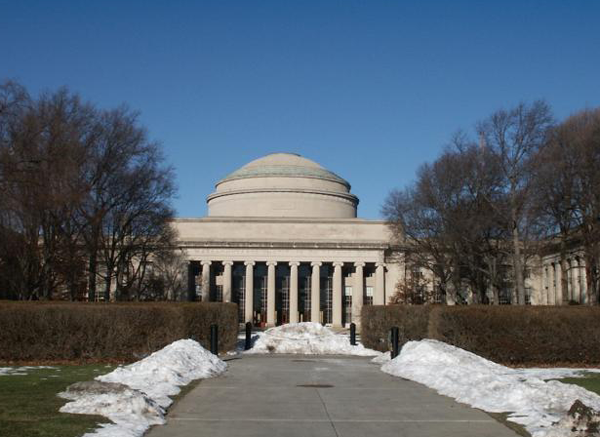
\includegraphics[width=0.9\columnwidth]{Figure1}
\caption{With Caption Below, be sure to have a good resolution image
  (see item D within the preparation instructions).}
\label{fig:figure1}
\end{figure}

\subsection{References and Citations}

Use a numbered list of references at the end of the article, ordered
alphabetically by first author, and referenced by numbers in brackets
\cite{ethics,
  Klemmer:2002:WSC:503376.503378,
  Mather:2000:MUT,
  Zellweger:2001:FAO:504216.504224}. For
papers from conference proceedings, include the title of the paper and
an abbreviated name of the conference (e.g., for Interact 2003
proceedings, use \textit{Proc. Interact 2003}). Do not include the
location of the conference or the exact date; do include the page
numbers if available. See the examples of citations at the end of this
document. Within this template file, use the \texttt{References} style
for the text of your citation.

Your references should be published materials accessible to the
public.  Internal technical reports may be cited only if they are
easily accessible (i.e., you provide the address for obtaining the
report within your citation) and may be obtained by any reader for a
nominal fee.  Proprietary information may not be cited. Private
communications should be acknowledged in the main text, not referenced
(e.g., ``[Robertson, personal communication]'').

\begin{table}
  \centering
  \begin{tabular}{|c|c|c|}
    \hline
    \tabhead{Objects} &
    \multicolumn{1}{|p{0.3\columnwidth}|}{\centering\tabhead{Caption --- pre-2002}} &
    \multicolumn{1}{|p{0.4\columnwidth}|}{\centering\tabhead{Caption --- 2003 and afterwards}} \\
    \hline
    Tables & Above & Below \\
    \hline
    Figures & Below & Below \\
    \hline
  \end{tabular}
  \caption{Table captions should be placed below the table.}
  \label{tab:table1}
\end{table}

\section{Sections}

The heading of a section should be in Helvetica 9-point bold, all in
capitals. Use Arial if Helvetica is not available. Sections should
not be numbered.

\subsection{Subsections}

Headings of subsections should be in Helvetica 9-point bold with
initial letters capitalized.  For
sub-sections and sub-subsections, a word like \emph{the} or \emph{of}
is not capitalized unless it is the first word of the heading.)

\subsubsection{Sub-subsections}

Headings for sub-subsections should be in Helvetica 9-point italic
with initial letters capitalized.  Standard {\textbackslash}section,
{\textbackslash}subsection, and {\textbackslash}subsubsection commands
will work fine.

\section{Figures/Captions}

Place figures and tables at the top or bottom of the appropriate
column or columns, on the same page as the relevant text
(see Figure~\ref{fig:figure1}). A figure or table may extend across both
columns to a maximum width of 17.78 cm (7 in.).

Captions should be Times New Roman 9-point bold.  They should be numbered (e.g.,
``Table~\ref{tab:table1}'' or ``Figure~\ref{fig:figure2}''), centered
and placed beneath the figure or table.  Please note that the words
``Figure'' and ``Table'' should be spelled out (e.g., ``Figure''
rather than ``Fig.'') wherever they occur.

Papers and notes may use color figures, which are included in the page
limit; the figures must be usable when printed in black and white in
the proceedings.  The paper may be accompanied by a short video figure
up to five minutes in length.  However, the paper should stand on its
own without the video figure, as the video may not be available to
everyone who reads the paper.

\section{Language, Style and Content}

The written and spoken language of SIGCHI is English. Spelling and
punctuation may use any dialect of English (e.g., British, Canadian,
US, etc.) provided this is done consistently. Hyphenation is
optional. To ensure suitability for an international audience, please
pay attention to the following:

\begin{itemize}
\item Write in a straightforward style.
\item Try to avoid long or complex sentence structures.
\item Briefly define or explain all technical terms that may be
  unfamiliar to readers.
\item Explain all acronyms the first time they are used in your text---e.g.,
``Digital Signal Processing (DSP)''.
\item Explain local references (e.g., not everyone knows all city
  names in a particular country).
\item Explain ``insider'' comments. Ensure that your whole audience
  understands any reference whose meaning you do not describe (e.g.,
  do not assume that everyone has used a Macintosh or a particular
  application).
\item Explain colloquial language and puns. Understanding phrases like
  ``red herring'' may require a local knowledge of English.  Humor and
  irony are difficult to translate.
\item Use unambiguous forms for culturally localized concepts, such as
  times, dates, currencies and numbers (e.g., ``1-5-97'' or ``5/1/97''
  may mean 5 January or 1 May, and ``seven o'clock'' may mean 7:00 am or
  19:00).  For currencies, indicate equivalences---e.g., ``Participants
  were paid 10,000 lire, or roughly \$5.''
\item Be careful with the use of gender-specific pronouns (he, she)
  and other gendered words (chairman, manpower, man-months). Use
  inclusive language that is gender-neutral (e.g., she or he, they,
  s/he, chair, staff, staff-hours,
  person-years). See~\cite{Schwartz:1995:GBF} for further advice and
  examples regarding gender and other personal attributes.
\item If possible, use the full (extended) alphabetic character set
  for names of persons, institutions, and places (e.g.,
  Gr{\o}nb{\ae}k, Lafreni\'ere, S\'anchez, Universit{\"a}t,
  Wei{\ss}enbach, Z{\"u}llighoven, \r{A}rhus, etc.).  These characters
  are already included in most versions of Times, Helvetica, and Arial
  fonts.
\end{itemize}

\section{Accessibility}
The Executive Council of SIGCHI has committed to making SIGCHI conferences more inclusive for researchers, practitioners, and educators with disabilities. As a part of this goal, the all authors are asked to work on improving the accessibility of their submissions. Specifically, we encourage authors to carry out the following five steps:
\begin{enumerate}
	\item Add alternative text to all figures
	\item Mark table headings
	\item Add tags to the PDF
	\item Verify the default language
	\item Set the tab order to ``Use Document Structure''
\end{enumerate}
Unfortunately good tools do not yet exist to create tagged PDF files from Latex. LaTeX users will need to carry out all of the above steps in the PDF directly using Adobe Acrobat, after the PDF has been generated.
 
For more information and links to instructions and resources, please see:
{\url{http://chi2014.acm.org/authors/guide-to-an-accessible-submission}}.

\section{Page Numbering, Headers and Footers}

Please submit your anonymous version for reviewing with page numbers
centered in the footer.  These must be removed in the final version of
accepted papers, as page numbers, headers, and footers will be added
by the conference printers.  Comment out the {\textbackslash}pagenumbering
command at the top of the document to remove page numbers.

\section{Producing and Testing PDF Files}

We recommend that you produce a PDF version of your submission well
before the final deadline.  Your PDF file must be ACM DL
Compliant. The requirements for an ACM Compliant PDF are available at:
{\url{http://www.sheridanprinting.com/typedept/ACM-distilling-settings.htm}}.

Test your PDF file by viewing or printing it with the same software we
will use when we receive it, Adobe Acrobat Reader Version 7. This is
widely available at no cost from~\cite{acrobat}.  Note that most
reviewers will use a North American/European version of Acrobat
reader, which cannot handle documents containing non-North American or
non-European fonts (e.g. Asian fonts).  Please therefore do not use
Asian fonts, and verify this by testing with a North American/European
Acrobat reader (obtainable as above). Something as minor as including
a space or punctuation character in a two-byte font can render a file
unreadable.

\section{Blind Review}

For archival submissions, CHI requires a ``blind review.'' To prepare
your submission for blind review, remove author and institutional
identities in the title and header areas of the paper. You may also
need to remove part or all of the Acknowledgments text.  Further
suppression of identity in the body of the paper and references is
left to the authors' discretion. For more details, see the submission
guidelines and checklist for your submission category.

\section{Conclusion}

It is important that you write for the SIGCHI audience.  Please read
previous years' Proceedings to understand the writing style and
conventions that successful authors have used.  It is particularly
important that you state clearly what you have done, not merely what
you plan to do, and explain how your work is different from previously
published work, i.e., what is the unique contribution that your work
makes to the field?  Please consider what the reader will learn from
your submission, and how they will find your work useful.  If you
write with these questions in mind, your work is more likely to be
successful, both in being accepted into the Conference, and in
influencing the work of our field.

\section{Acknowledgments}

We thank CHI, PDC and CSCW volunteers, and all publications support
and staff, who wrote and provided helpful comments on previous
versions of this document.  Some of the references cited in this paper
are included for illustrative purposes only.  \textbf{Don't forget
to acknowledge funding sources as well}, so you don't wind up
having to correct it later.

% Balancing columns in a ref list is a bit of a pain because you
% either use a hack like flushend or balance, or manually insert
% a column break.  http://www.tex.ac.uk/cgi-bin/texfaq2html?label=balance
% multicols doesn't work because we're already in two-column mode,
% and flushend isn't awesome, so I choose balance.  See this
% for more info: http://cs.brown.edu/system/software/latex/doc/balance.pdf
%
% Note that in a perfect world balance wants to be in the first
% column of the last page.
%
% If balance doesn't work for you, you can remove that and
% hard-code a column break into the bbl file right before you
% submit:
%
% http://stackoverflow.com/questions/2149854/how-to-manually-equalize-columns-
% in-an-ieee-paper-if-using-bibtex
%
% Or, just remove \balance and give up on balancing the last page.
%
\balance

\section{References format}
References must be the same font size as other body text.
% REFERENCES FORMAT
% References must be the same font size as other body text.

\bibliographystyle{acm-sigchi}
\bibliography{sample}
\end{document}
